%%%% acra.tex

\typeout{ACRA Instructions for Authors}

% This is the instructions for authors for ACRA.
\documentclass{article}
\usepackage{acra}
\usepackage{lmodern}% http://ctan.org/pkg/lm
\usepackage{amsmath}
\usepackage{graphicx}
\usepackage{color}
\usepackage{hyperref}
\usepackage{amssymb}
\usepackage{url}
\usepackage{pdfpages}
\usepackage{fancyhdr}
\usepackage{subfig}
\usepackage{listings} 
\usepackage{selinput}    

% The file acra.sty is the style file for ACRA. 
% The file named.sty contains macros for named citations as produced 
% by named.bst.

% The preparation of these files was supported by Schlumberger Palo Alto
% Research, AT\&T Bell Laboratories, and Morgan Kaufmann Publishers.
% Shirley Jowell, of Morgan Kaufmann Publishers, and Peter F.
% Patel-Schneider, of AT\&T Bell Laboratories collaborated on their
% preparation. 

% These instructions can be modified and used in other conferences as long
% as credit to the authors and supporting agencies is retained, this notice
% is not changed, and further modification or reuse is not restricted.
% Neither Shirley Jowell nor Peter F. Patel-Schneider can be listed as
% contacts for providing assistance without their prior permission.

% To use for other conferences, change references to files and the
% conference appropriate and use other authors, contacts, publishers, and
% organizations.
% Also change the deadline and address for returning papers and the length and
% page charge instructions.
% Put where the files are available in the appropriate places.

\title{Stick-Breaking Process and Dirichlet Process}
\author{Diego Garrido}

\begin{document}

\maketitle
\href{https://nbviewer.jupyter.org/github/dgarridoa/dirichlet_process/blob/master/Dirichlet_Process.ipynb}{\color{blue}{Jupyter Notebook}}
\section{Dirichlet Distribution}

A multivariate generalization of the beta distribution is the Dirichlet distribution, which has support over the probability simples, defined by

\begin{align}
\triangle_{K} = \{C: C_{k}\geq 0, \sum_{k=1}^{K}C_{k}=1\}
\end{align}

The pdf is defined as follows:

\begin{align}
Dir(C|\alpha) \triangleq \frac{\prod_{k=1}^{K}C_{k}^{\alpha_{k}-1}\mathbb{I}(C \in \triangle_{K})}{B(\alpha)}
\end{align}

In Figure 1 we have samples from a symmetric Dirichlet Distribution, lower $\alpha$ results in very sparse distribution, with many zeros and high variance, while higher $\alpha$ makes the size of the atoms more similar with higher density in the center of the simplex, note that with $\alpha=1$ the distribution is uniform over the simplex (i.e. no region with higher density). In addition, a higher dimension results in less variance and decrease in the size of the atom because there are more dimensions over which the mass must be distributed.\\

\begin{figure}[h]
\centering
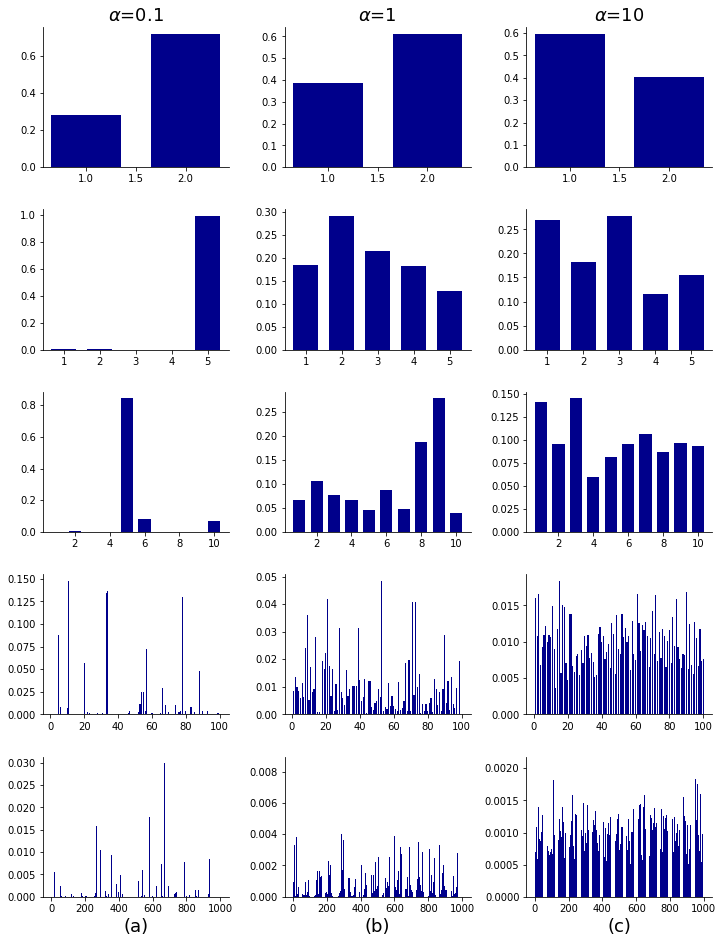
\includegraphics[scale=0.3]{img/dirichlet_samples.png}  
\caption{Samples from a symmetric Dirichlet Distribution, that is $Dir(\frac{\alpha}{K}1_{K})$, with $\alpha\in\{0.1, 1, 1\}$ and $K\in\{2, 5, 10, 100, 1000\}$.}
\end{figure}

\section{Dirichlet Process}

We use the stick-breaking point construction of a Dirichlet Process. If $\alpha>0$ and if $G$ is a probability measure on $\Omega_{\phi}$ the random discrete probability measure $\Theta:=\sum C_{k}\delta_{\Phi_{k}}$ generated by

\begin{align}
& V_{1}, V_{2}, \ldots \sim_{iid} Beta(1, \alpha)\\
& C_{k} = V_{k}\prod_{j=1}^{k-1}(1-V_{k})\\
& \Phi_{1}, \Phi_{2}, \ldots \sim_{iid} G_{0}
\end{align}

is called a Dirichlet Process (DP) with base measure $G$ and concentration paremeter $\alpha>0$, and we denote its law by $DP(\alpha, G_{0})$. In practice, when we sample from this distribution we need to add a tolerance (1e-8) so that the process ends in a reasonable number of steps.\\

In Figure 2 we have some samples from a stick-breaking process (left) and dirichlet process  (right) with base measure $\mathcal{N}(0, 1)$ with concentration parameter $\alpha\in\{0.1, 0.2, 0.6, 6, 60\}$. The higher the alpha, the less variance and the greater number of atoms, on the contrary, small values of alpha show a high variance and a lower number of atoms, additionally they show a greater variance in the number of atoms according to the random seed.\\

\begin{figure}[h]
\centering
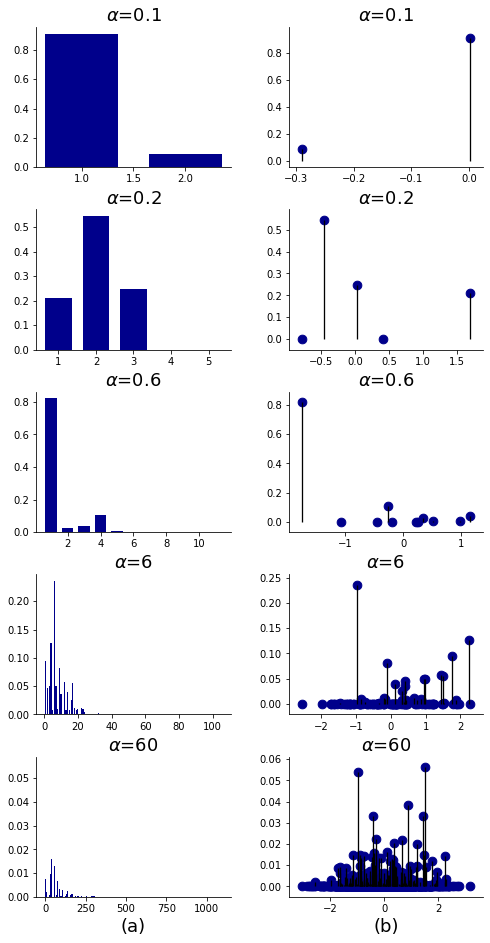
\includegraphics[scale=0.3]{img/dp_samples.png}  
\caption{Random measures sample from a Dirichlet process with normal base measure $\mathcal{N}(0,1)$ with concentration parameter $\alpha\in\{0.1, 0.2, 0.6, 6, 60\}$. \textit{(a)} Samples from stick-breaking process. \textit{(b)} Samples from Dirichlet process with those mixture weights.}
\end{figure}

We want to sample from $\Theta \sim Dir(\alpha, G)$ by $N$ times:

\begin{align}
\Theta := \sum C_{k}\delta_{\Phi_{k}}
\end{align}

from the stick-breaking process we know $C_{1:K}$ and $\Phi_{1:K}$, where $K$ is finite with probability 1, then we can sample from this discrete distribution a sequence $\phi_{1}, \phi_{2}, \ldots$ by:

\begin{align}
L_{i}\sim Mult(C)\\
\phi_{i} = \Phi_{L_{i}}
\end{align}

In Figure 3 we have some samples from random measures sampled from a Dirichlet Process. To higher $N$ the possibility of repeating a previous $\phi$ is greater and this occurs with greater probability for smaller $\alpha$, this is because the number of possibilities/atoms is less. In addition, to higher $N$ the empirical distribution converge to the true discrete distribution.\\

\begin{figure}[h]
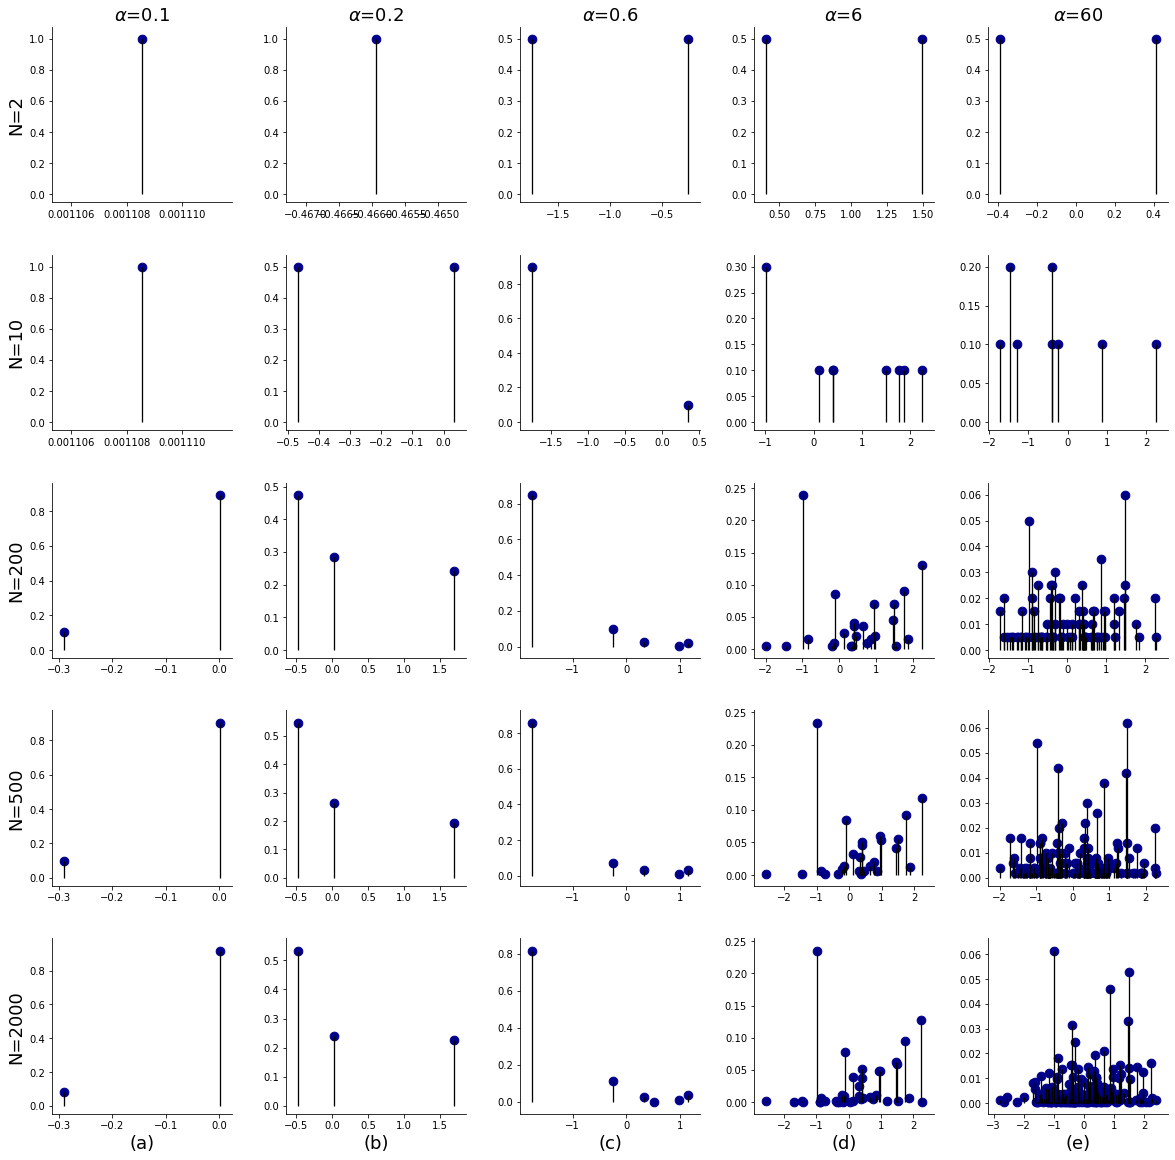
\includegraphics[scale=0.2]{img/g_samples.png}  
\caption{Samples from random measures samples from a Dirichlet Process with ormal base measure $\mathcal{N}(0,1)$ with concentration parameter $\alpha\in\{0.1, 0.2, 0.6, 6, 60\}$. The atom sizes is normalized based on the number of samples.}
\end{figure}

\end{document}